\documentclass[../doc.tex]{subfiles}

\begin{document}
\section{Réalisation de l'intelligence artificielle}
Plus spécifique au mécaniques de l'intelligence artifielle,
 trois types de personnages e doivent être implémentés à la carte:
\begin{itemize}
    \item Des IA qui restent bloqués sur place et qui discutent en groupe
    \item Des IA qui se déplacent de manière aléatoire (ou qui patrouillent)
    \item Des NPC qui effectuent des animations précises
        (juste pour le décor plus réaliste et travaillé)
\end{itemize}

Pour créer l'IA, nous utiliserons un système de Nav Mesh, zone où les NPC peuvent naviguer pour aller d'un point A vers un point B.
Nous avons déjà réalisé une IA qui selon une liste de positions, se balade d'un point à un autre avant de revenir à sa position initiale.

\begin{figure}
    \centering
    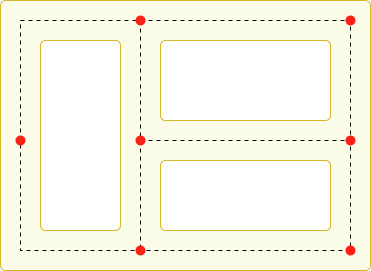
\includegraphics[scale=0.5]{NavPatrolMaze.jpg}
    \caption{Schéma d'un mouvement de patrouille}
\end{figure}

\end{document}
